\subsection{Reputation Scoring}
Reputation Scores are generated using two python scripts. One for reputation scoring posts and another for reputation scoring users. The scripts will each be scheduled to automatically run periodically and require no external intervention to execute. Each script will first establish a connection to the database using the mysql.connector library [39]. The library contains several functions to interact with the database. Once a connection is established, the database is queried and the results of those queries are used in the script to generate reputation scores for each post or user in the system (depending on the script). These scores are then normalised between 0 and 1 and then the database is updated with these newly calculated reputation scores using the database connection created earlier. The connection is then closed before the script terminates.

\subsubsection{Reputation Scoring for Posts}
Once a connection to the database has been established, the database must be queried to return a table with the values required to score the reputation of each post. These values are: The number of comments on the post, the number of upvotes on the post and the number of downvotes on the post. Figure \ref{fig:PostRepQuery} shows the query used to attain these values. The query selects 3 attributes from the comments table, grouped by the post id. The comments table is used because every post in the system is treated as a `root comment'. The first attribute, `comments' finds the number of entries in this table with the id of the post, subtracting 1 since the post itself must be discounted. The `upvotes' and 	`downvotes' attributes are found simply by finding those values from the comments table. Note that the query also performs the weighting needed for the summation of these attributes in the algorithm.

\begin{figure}[H]
\centering
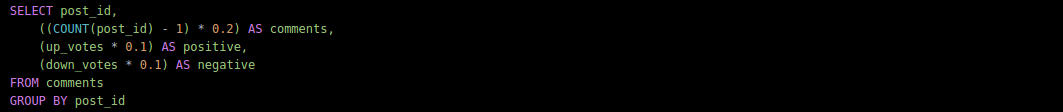
\includegraphics[height=1in]{Images/Implementation/PostRepQuery}
\caption{Query for selecting values for reputation scoring of posts}
\label{fig:PostRepQuery}
\end{figure}

Upon the conclusion of this query, the result will be a table similar to that shown in Figure \ref{fig:PostRepTable}.

\begin{figure}[H]
\centering
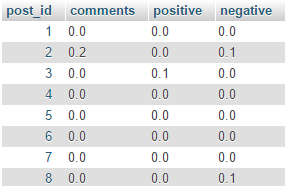
\includegraphics[height=1.5in]{Images/Implementation/PostRepTable}
\caption{Table showing example values for reputation scoring of posts}
\label{fig:PostRepTable}
\end{figure}

The python script will then iterate through each row of the result of this query. For each row, the script will perform the summation of the weighted values (comments, positive and negative) to get a reputation value. Note that the `negative' value for each post is subtracted instead of added to comply with the desired weightings. These values are all then inserted into a pandas dataframe \cite{Pandas} along with their respective post id. This is shown in Figure \ref{fig:PostRepPython1}.

\begin{figure}[H]
\centering
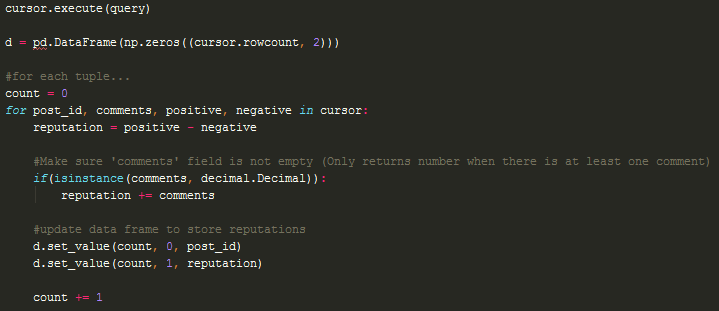
\includegraphics[width=\linewidth]{Images/Implementation/PostRepPython1}
\caption{Python code for calculating post reputation scores}
\label{fig:PostRepPython1}
\end{figure}

The script will now find the maximum and minimum reputation scores of all of the users as shown in Figure \ref{fig:PostRepPython1}. If this difference is 0, it must follow that every single post has the exact same reputation score (An unlikely scenario for the Fidelis system due to the large number of intended users). If this is the case, all of the posts will have their reputations scaled to 0. If this difference is not 0, a Python lambda function is used to normalise all reputation scores between 0 and 1. This lambda function is applied to the entire dataframe column, rather than iterating over each one individually.

\begin{figure}[H]
\centering
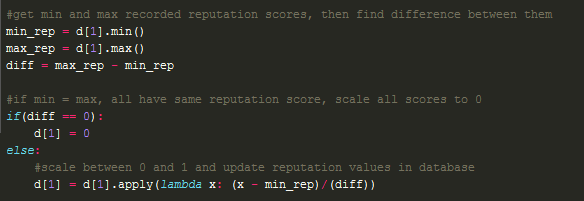
\includegraphics[width=\linewidth]{Images/Implementation/PostRepPython2}
\caption{Python code for normalising post reputation scores}
\label{fig:PostRepPython2}
\end{figure}

Finally, as shown in Figure \ref{fig:PostRepPython3}, the script runs through each row of the dataframe and updates the reputation score of each post using the final, normalised reputation score and the associated post id. This is done in the form of an SQL update query which is then committed to the database. Once each post has been assigned a new score, the database connection is terminated along with the script.

\begin{figure}[H]
\centering
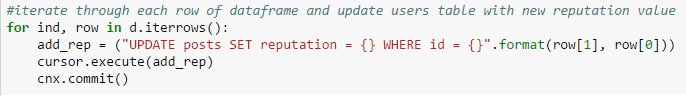
\includegraphics[width=\linewidth]{Images/Implementation/PostRepPython3}
\caption{Python code for inserting post reputation scores into the database}
\label{fig:PostRepPython3}
\end{figure}

\subsubsection{Reputation Scoring for Users}
Once a connection to the database has been established, the database must be queried to return a table with the values required to score the reputation of each user. These values are: the number of upvotes on all of the user's posts, the number of downvotes on all of the user's posts, the number of comments on all of the user's posts, the number of upvotes on all of the user's comments, the number of downvotes on all of the user's comments and the number of followers a user has. Figure \ref{fig:UserRepQuery} shows the query used to attain these values. The query selects 4 attributes from the various tables, using a number of joins. In total, the query joins together 3 separate subqueries. The first subquery finds the weighted number of upvotes on all of the user's comments and posts as well as the weighted number of downvotes on all of the user's comments. The next subquery will find the weighted number of comments on all of the users posts, where the comment isn't a `root comment' (i.e. a post) and the user id on the comment is not that of the user whose reputation is being scored. This avoids a user potentially creating many comments on their own posts simply to `boost' their reputation score.

\begin{figure}[H]
\centering
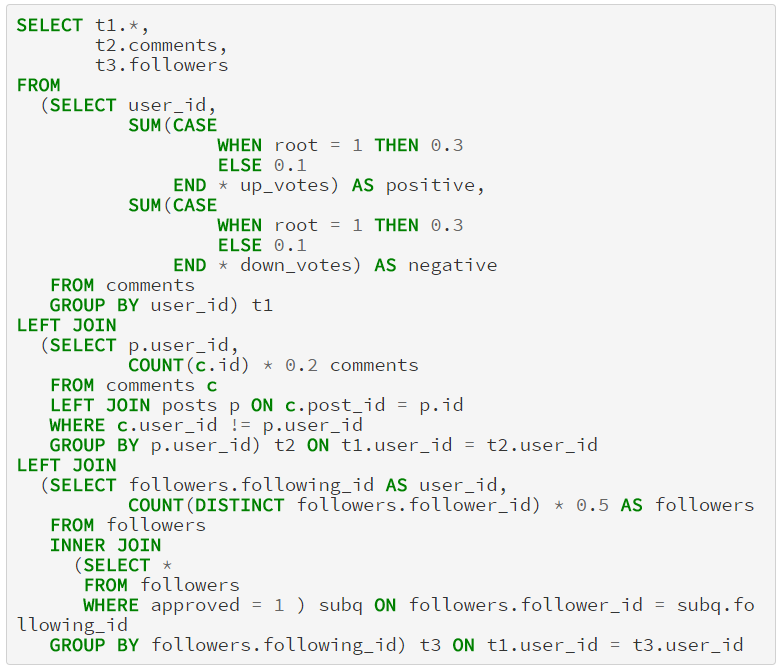
\includegraphics[height=4in]{Images/Implementation/UserRepQuery}
\caption{Query for selecting values for reputation scoring of users}
\label{fig:UserRepQuery}
\end{figure}

Upon the conclusion of this query, the result will be a table similar to that shown in Figure \ref{fig:UserRepTable}.

\begin{figure}[H]
\centering
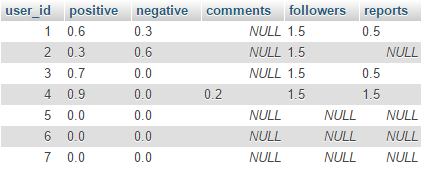
\includegraphics[height=1.5in]{Images/Implementation/UserRepTable}
\caption{Table showing example values for reputation scoring of users}
\label{fig:UserRepTable}
\end{figure}

The python script will then iterate through each row of the result of this query. For each row, the script will perform the summation of the weighted values (positive, negative, comments and followers) to get a reputation value. Note that the `negative' value for each user is subtracted instead of added to comply with the desired weightings. These values are all then inserted into a pandas dataframe \cite{Pandas} along with their respective user id. This is shown in Figure \ref{fig:UserRepPython1}.

\begin{figure}[H]
\centering
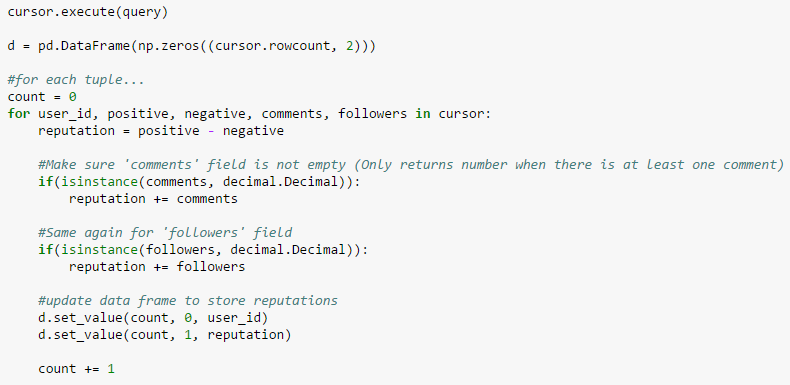
\includegraphics[width=\linewidth]{Images/Implementation/UserRepPython1}
\caption{Python code for calculating user reputation scores}
\label{fig:UserRepPython1}
\end{figure}

The script will now find the maximum and minimum reputation scores of all of the users as shown in, using the same method demonstrated for normalising the reputation scores for posts. On completion of this normalisation, every reputation score will be between 0 and 1. Finally, as shown in Figure \ref{fig:UserRepPython2}, the script runs through each row of the dataframe and updates the reputation score of each user using the final, normalised reputation score and the associated user id. This is done in the form of an SQL update query which is then committed to the database. Once each user has been assigned a new score, the database connection is terminated along with the script.

\begin{figure}[H]
\centering
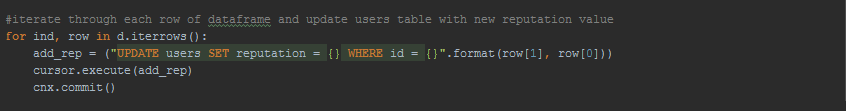
\includegraphics[width=\linewidth]{Images/Implementation/UserRepPython2}
\caption{Python code for normalising user reputation scores}
\label{fig:UserRepPython2}
\end{figure}